\section{Convolutional Neural Network: U-Net}
\label{sec:Model}
Zur Verarbeitung von Bildern haben sich in der Vergangenheit Convolutional Neural Networks (CNNs) bewiesen.
Grundsätzlich besteht ein CNN aus mehreren Convolutional Layers, gefolgt von einem Pooling Layer.
Wird von einem tiefen CNN gesprochen, so ist damit ein Netzwerk aus mehreren CNN-Einheiten gemeint.
\\
Das hier verwendete U-Net gehört zu den tiefen CNNs und besitzt eine U-förmige Struktur.
Das U-Net gewann $2015$ zwei Challanges, zum einen für automatische Computerdetektion von Karies in Bissflügel-Röntgenaufnahmen (ISBI $2015$) und zum anderen die Erkennung von Zellen (ISBI $2015$).\cite{RFB15a}

\subsection{Architektur}
Die verwendete Netzwerkstruktur ist in \autoref{tab:structure} aufgeführt und in \autoref{fig:unet_structure} visuell dargestellt.
Das U-Net besteht dabei aus einem absteigenden und einem aufsteigenden Ast, ähnlich wie bei einem Auto-Encoder.
Zusätzlich sind Layers aus dem Encoder direkt mit Layers aus dem Decoder verknüpft (siehe Pfeile in gen. Abb.).
Die Daten werden hier lediglich kopiert und über das Layer 'Concatenate' mit den vorherigen Daten zusammengefügt.
\\
Um das Übertrainieren des Netzes zu verhindern, wird in jeder CNN-Einheit ein Dropout verwendet.
Der Dropout steigt mit $0.1$ pro CNN-Einheit für den aufsteigenden Ast bzw. mit der Tiefe des Netzes.
Der maximale Dropout liegt bei der mittleren CNN-Einheit vor.
Bei dem aufsteigendem Ast wird der Dropout wieder um $0.1$ je CNN-Einheit reduziert.
\\
Analog dazu wird die Filtergröße des 'Convolutional Layers' mit der tiefe pro Einheit verdoppelt bzw. beim aufsteigenden Teil halbiert.
Im Ouput-Layer wird die Sigmoid-Funktion und in den restlichen Convolutional Layers die Rectifier Aktivierungsfunktion (ReLU) verwendet.
\\
Zudem wird Adam als Optimizer festgelegt.
'Binary Crossentropy' wird hier als Verlustfunktion eingesetzt, da diese eine gute Wahl für Klassifizierungsprobleme mit zwei Klassen ($0$/Land oder $1$/Wasser) ist.
Das Modell wird über die 'Accuracy' bewertet, d.h. der Anteil der übereinstimmenden Pixel der vorhergesagten Bilder mit der Maske.
\\
Es müssen insgesamt $\SI{609895}{\text{Parameter}}$ trainiert werden.
Die Wahl der Hyperparameter wird im nächsten Abschnitt (\autoref{sec:Hyperparameter}) erläutert.
\begin{figure}
    \centering
    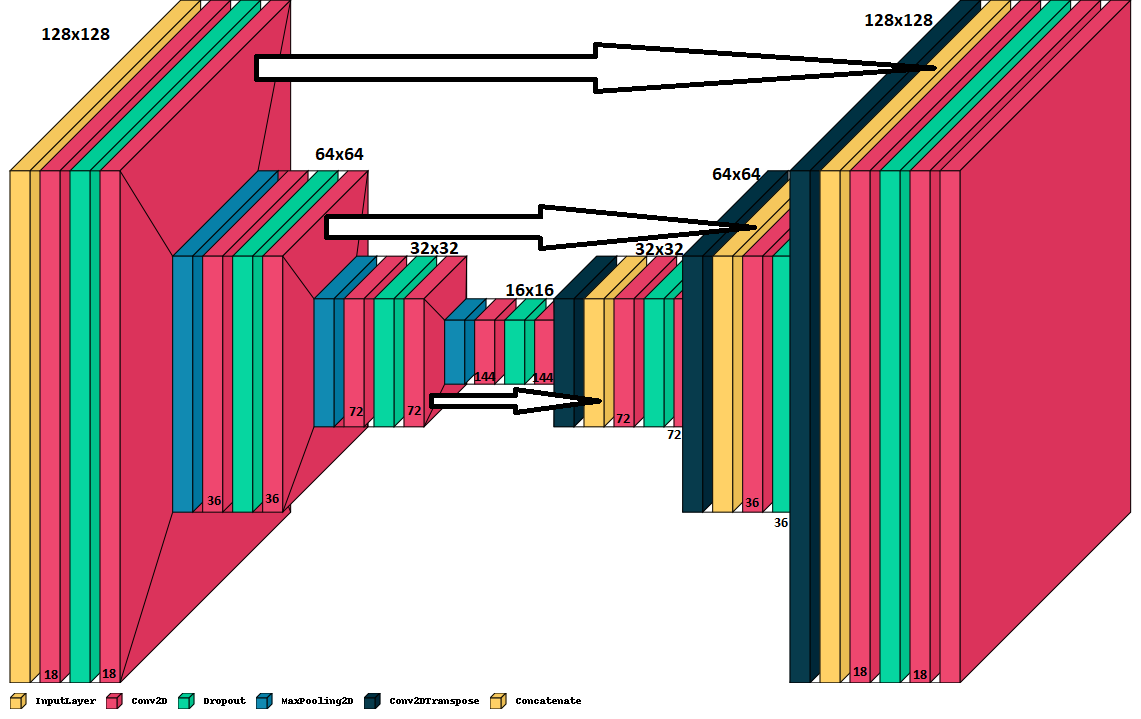
\includegraphics[width=0.8\textwidth]{content/img/unet_struc_bearbeitet_2.png}
    \caption{Schematische Darstellung der verwendeten Netzwerkstruktur: U-net. (VisualKeras)}
    \label{fig:unet_structure}
\end{figure}

\begin{table}
    \centering
    \caption{Netzwerk Struktur: U-Net}
    \label{tab:structure}
    \begin{tabular}{l c l}
        \toprule
        Layers & Output Dim. & Parameter \\
        \midrule
        Conv 2D                 & $(128, 128, 18)$ & $504$ \\       
        Dropout               & $(128, 128, 18)$ & $0  $ \\       
        Conv 2D               & $(128, 128, 18)$ & $2934  $ \\       
        Max Pooling 2D    & $(64, 64, 18)  $ & $0  $ \\       
        & & \\ 
        Conv 2D               & $(64, 64, 36)  $ & $5868  $ \\       
        Dropout             & $(64, 64, 36)  $ & $0  $ \\       
        Conv 2D               & $(64, 64, 36)  $ & $11700 $ \\       
        Max Pooling 2D  & $(32, 32, 36)  $ & $0  $ \\       
        & & \\ 
        Conv2D               & $(32, 32, 72)  $ & $23400 $ \\       
        Dropout             & $(32, 32, 72)  $ & $0  $ \\       
        Conv 2D               & $(32, 32, 72)  $ & $46728 $ \\       
        Max Pooling 2D  & $(16, 16, 72)  $ & $0  $ \\       
        & & \\ 
        Conv 2D               & $(16, 16, 144) $ & $93456 $ \\       
        Dropout             & $(16, 16, 144) $ & $0  $ \\       
        conv 2D               & $(16, 16, 144) $ & $186768$ \\       
        Conv 2D Transpose & $(32, 32, 72)  $ & $41544 $ \\       
        Concatenate       & $(32, 32, 144) $ & $0  $ \\
        & & \\             
        Conv 2D               & $(32, 32, 72)  $ & $93384 $ \\       
        Dropout             & $(32, 32, 72)  $ & $0  $ \\       
        Conv 2D               & $(32, 32, 72)  $ & $46728 $ \\       
        Conv 2D Transpose & $(64, 64, 36)  $ & $10404 $ \\       
        Concatenate     & $(64, 64, 72)  $ & $0  $ \\                             
        & & \\             
        Conv 2D             & $(64, 64, 36)  $ & $23364 $ \\       
        Dropout             & $(64, 64, 36)  $ & $0  $ \\       
        Conv 2D              & $(64, 64, 36)  $ & $11700 $ \\       
        Conv 2D Transpose & $(128, 128, 18)$ & $2610  $ \\       
        Concatenate     & $(128, 128, 36)$ & $0  $ \\
        & & \\             
        Conv 2D             & $(128, 128, 18)$ & $5850  $ \\       
        Dropout             & $(128, 128, 18)$ & $0  $ \\       
        Conv 2D              & $(128, 128, 18)$ & $2934  $ \\       
        Conv 2D              & $(128, 128, 1) $ & $19 $ \\
        \hline
        Gesamtanzahl: & & $\SI{609895}{}$ \\
        \bottomrule
    \end{tabular}
\end{table}

\FloatBarrier

\subsection{Optimierung der Hyperparameter}
\label{sec:Hyperparameter}
Zur Bestimmung der optimalen Hyperparameter wird eine zufällige Gittersuche durchgeführt.
D.h. es werden zufällige Parameter aus einem Parameterraum gezogen und darauf das Modell trainiert und evaluiert.
Auf eine vollständige Gittersuche wird aufgrund der hohen Rechenzeit verzichtet.
\\
Die Gittersuche wird auf einer Teilstichprobe mit $9000$ Bildern durchgeführt.
Dabei werden $2/3$ der Daten zum trainieren bzw. validieren verwendet und $1/3$ als Testdatensatz.
Die Validierungs- und Trainingsdaten werden gleichmäßig aufgeteilt (jeweils $\SI{50}{\percent}$).
\\
Folgende Parameter können Werte im angegebenen Intervall (I) bzw. Parameterraum (P) annehmen:
\begin{itemize}
    \item U-Net-Struktur: Level der Tiefe P$[3, 4, 5, 6]$
    \item Lernrate aus Intervall I$[0.0001, 0.01]$
    \item Filteranzahl (Conv 2D): Startwert I$[3, 33]$
    \item Kernel-Größe (Conv 2D) P$[2, 3, 4]$
    \item Kernel initializer (Conv 2D) P$[$He Normal, Glorot Uniform$]$
    \item Dropout Startwert I$[0.0, 0.5]$
\end{itemize}
Insgesamt wurden $100$ Modelle mit einer Batchsize von $128$ und Epochenanzahl von $20$ trainiert und ausgewertet.
Die Ergebnisse der einzelnen Parameter sind in \autoref{fig:grid_ergebnisse} graphisch dargestellt.
\begin{figure}
    \centering
    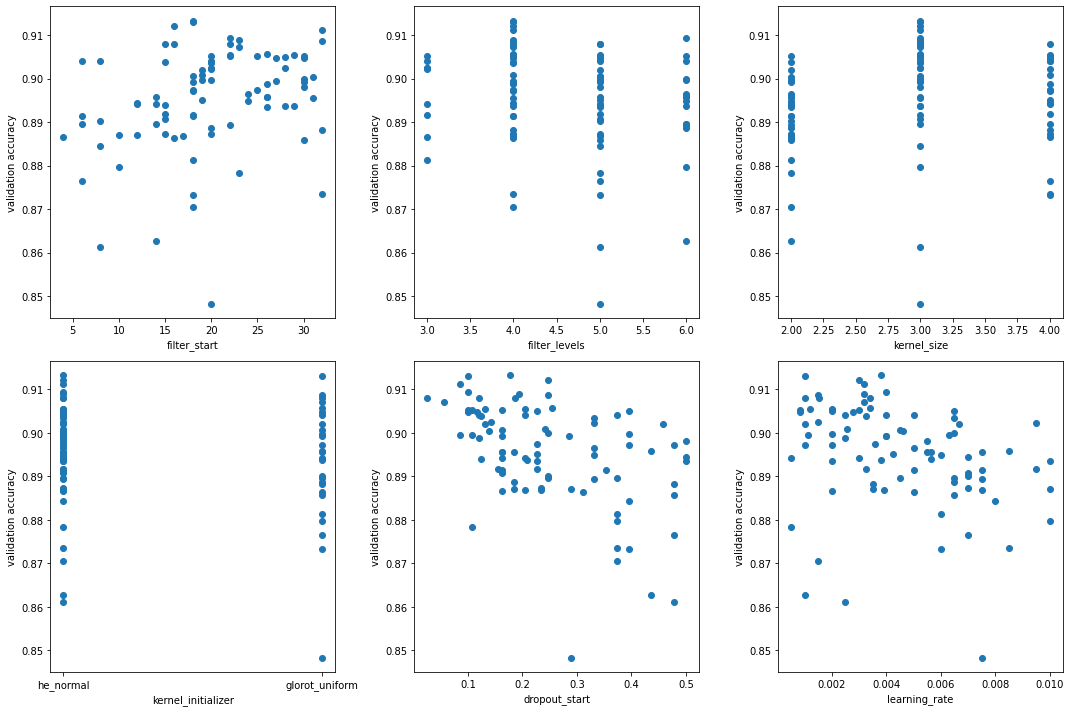
\includegraphics[width=0.8\textwidth]{content/img/grid_ergebnisse.png}
    \caption{Die Accuracy zu den sechs variierten Parametern der zufälligen Gittersuche.}
    \label{fig:grid_ergebnisse}
\end{figure}
\FloatBarrier
Die Wahl des 'Kernel Initializer' scheint kaum Einfluss auf die Accuracy zu haben.
Hingegen ist bei der Lernrate und beim Startwert der Dropoutrate und der Filter ein Trend zu erkennen.
Eine geringe Dropout- und Lernrate bzw. eine größere Filteranzahl deutet auf eine höhere Accuracy hin.
Ebenso sollte eine $3\times3$ Kernelgröße der Convolutional Layer und eine U-Net Tiefe von $4$ gewählt werden.

Das Modell mit der besten Accuracy auf den Validierungsdaten, wird nun auf allen Daten ($\sim \SI{60000}{}$) trainiert.

\subsection{Training}
%